% ex_cap0.tex
\chapter*{Apresentação}
\addcontentsline{toc}{chapter}{Apresentação}
\markboth{Apresentação}{Apresentação}   % cabeçalho, se usar pagestyle com cabeçalho

Em março de 2022 estava no InovaUSP, em São Paulo, para minha primeira visita ao Centro de Inteligência Artificial da Universidade de São Paulo (C4AI). Descobri o lugar por acaso. A inteligência artificial (IA) não fazia parte de meu projeto inicial de pesquisa de doutorado, mas um amigo, sabendo de meus novos interesses acadêmicos pelos estudos de ciência e tecnologia, enviou-me via WhatsApp uma notícia sobre a inauguração de um centro de pesquisas em IA instalado na USP. A mesma curiosidade que me levou a abrir aquele link motivou-me a escrever para João, coordenador do Observatório da Inteligência Artificial e Impacto Social (OBIA) do C4AI. Expliquei minhas intenções de pesquisa, mencionando as disciplinas sobre ciência e tecnologia que havia cursado e um texto de Kate Crawford e Vladan Joler sobre a Amazon Echo\footnote{O texto 
em questão, \emph{Anatomia de um sistema de inteligência artificial} \parencite{Crawford2018Anatomy}, foi um dos primeiros que li sobre  inteligência artificial e, de certa forma, inspirou-me a começar esta pesquisa. 
A versão original do mapa, em inglês, está disponível em: 
\url{https://anatomyof.ai}. A tradução brasileira, por Cristiana Gonzales 
e Pedro P. Ferreira, foi publicada pela revista \textit{ComCiência} 
(Unicamp/Labjor) em 20 de setembro de 2020 e está disponível em: 
\url{https://www.comciencia.br/anatomia-de-um-sistema-de-inteligencia-artificial/}. 
Acesso em: 6 abr. 2026.}

João me guiou pelas instalações físicas do Centro. Ao me aproximar da sala principal de convivência dos pesquisadores, notei que a porta estava fechada, mas uma parede inteira de vidro expunha todo o interior ao corredor. Parei ali por alguns instantes, observando através do vidro. Fileiras de computadores ocupavam estações de trabalho compartilhadas. Naquele dia, não havia ninguém na sala; ainda assim, a transparência seletiva daquele espaço me intrigou. Era possível imaginar os pesquisadores, acompanhar o trabalho que ali aconteceria, mas a porta fechada indicava que a entrada era controlada. Era um espaço parcialmente aberto: a parede de vidro permitia ver o interior, mas a porta controlava quem entrava. Será que era ali o ``laboratório do C4AI''? Pensava com a expectativa de encontrar tal lugar.

Enquanto caminhávamos pelos corredores, algo chamou minha atenção. Uma sala trancada que, através de uma pequena janela de vidro na porta de madeira, permitia vislumbrar um pouco do que havia em seu interior. Pareciam ser vários gabinetes de computadores que, mais tarde, eu descobriria tratar-se das unidades de processamento, as chamadas GPUs (\textit{Graphics Processing Units)} utilizadas para processar dados em alta velocidade e em paralelo, interligadas por uma extensa rede de cabeamento estruturado. No início desta pesquisa, em 2022, não era comum que imagens do interior de \textit{data centers} circulassem publicamente, e a quantidade de máquinas concentradas naquela sala era, para mim, algo inédito, uma materialidade da computação que o uso cotidiano de computadores pessoais e sistemas de inteligência artificial raramente traz à tona.\footnote{Ursula K. Le Guin, em ensaio de 2005, criticava o uso da palavra \enquote{tecnologia} como sinônimo exclusivo de alta tecnologia: \textit{Technology is the active human interface with the material world}. Texto disponível em: \url{https://www.ursulakleguin.com/a-rant-about-technology}, acesso em: 21 jan. 2026. A IA começa na extração mineral, na fabricação de cristais de silício, na circulação da eletricidade através de transistores, e essa cadeia de mediações não aparece no uso cotidiano dos sistemas. Como Lécuyer e Brock demonstram, as histórias convencionais da microeletrônica são \textit{under materialized}: focam excessivamente no design de dispositivos e deixam de lado as redes centradas na produção e manipulação de materiais semicondutores \parencite{LecuyerBrock2006Materiality}. Em certo sentido, ensinou-se pedras a fazer cálculos, e cálculos a escrever e a criar imagens.} Perguntei se aquela sala era o laboratório do Centro. Afinal, ali estavam as máquinas potentes que eu esperava encontrar. Mas não havia cientistas trabalhando, nem qualquer atividade humana visível; as GPUs estavam ali, estáticas, sozinhas, e o único movimento era o piscar rítmico de suas luzes. João disse que não, explicou que era como se fosse a área de TI (Tecnologia da Informação) do Centro. Respondi com um ``Ah!'' monossilábico, com certo constrangimento, e seguimos caminhando.

A situação, no entanto, acabou se transformando em um \textit{problema} de pesquisa\footnote{A noção remete ao convite de Donna Haraway, em \textit{Staying with the Trouble}, para \enquote{ficar com o problema}. Não encontrar o laboratório e os cientistas não é um problema a ser resolvido. É um problema que a pesquisa tensiona ao longo do tempo sem a pretensão de oferecer uma resolução ou uma resposta permanente \parencite{Haraway2016Staying}.}: \textit{onde está o laboratório de IA e onde estão os seus cientistas?} Eu tinha a expectativa de encontrar um lugar cheio de supercomputadores e cientistas desenvolvendo pesquisa em inteligência artificial. Mas eles não estavam lá, nem estiveram pelos anos seguintes de realização desta pesquisa. Havia uma sala com infraestrutura de microprocessadores para treinar modelos de IA e outra com computadores de mesa para uso dos pesquisadores, onde às vezes eu encontrava alguns deles, mas nunca ficavam por muito tempo. A pandemia de Covid-19 havia acabado de recuar, mas o padrão se manteria ao longo dos quase quatro anos que se seguiram, o laboratório continuaria existindo de forma não centralizada e os pesquisadores trabalham remotamente, compartilhando infraestruturas computacionais acessadas à distância.\footnote{Durante a entrevista com Fábio, diretor do Centro, ele também comentou esse aspecto distribuído quando mencionei que raramente via pesquisadores reunidos no espaço. Fábio observou: \enquote{A gente começou o centro na pandemia e depois as pessoas passaram a vir menos no local de trabalho [...] Eu sinto falta de um pouco de mais conexão [...] Antes da pandemia era mais forte. [...] quando o C4AI começou, eu tinha muita dúvida de como a gente ia conseguir fazer um centro tão disperso, tanta gente em tanto lugar. Isso não foi dificuldade nenhuma.} Essa reflexão orienta a discussão sobre o laboratório distribuído desenvolvida nos capítulos seguintes desta tese.}

Oito meses depois, em 30 de novembro de 2022, a OpenAI lançou o ChatGPT, disponibilizado gratuitamente como \enquote{pesquisa prévia}. O \textit{chat} ganhou popularidade rapidamente e atingiu mais de 1 milhão de usuários em cinco dias. A inteligência artificial deixava de ser objeto de pesquisa de círculos acadêmicos especializados e se tornava fenômeno de massa, presente nos debates públicos e nas manchetes de jornal. Enquanto isso, o laboratório que eu visitara em março continuava operando silenciosamente: os cientistas seguiam trabalhando remotamente, as GPUs processavam modelos, as mesas permaneciam vazias. A explosão pública da IA generativa não alterou a rotina de pesquisa do C4AI; intensificou, porém, o estranhamento da minha pergunta inicial. Se a IA parecia estar em quase todo lugar, nos \textit{smartphones} e nas conversas de não-especialistas, onde exatamente estava o laboratório que a produzia? Para entender isso, como descobriria, teria que investigar o que \enquote{laboratório} e \enquote{fazer tecnociência} querem dizer nesse contexto. 

Para investigar o que é um laboratório de IA e como os pesquisadores do C4AI fazem IA, \textit{segui} cientistas e engenheiros em ação \parencite{Latour1987Science}.\footnote{O subtítulo desta tese, \textit{como seguir cientistas e engenheiros --- universidade afora}, é uma variação do subtítulo de \textit{Ciência em Ação}, \textit{como seguir cientistas e engenheiros sociedade afora}. Nesse deslocamento, \enquote{sociedade afora} dá lugar a \enquote{universidade afora}, e o travessão marca a passagem do dentro para o fora do Centro. Dessa maneira, retomo a primeira regra de método de Latour, que consiste em \textit{seguir} cientistas e engenheiros nos momentos e locais em que produzem fatos e máquinas (tecnociência). Faço isso, contudo, a partir de um centro de pesquisa universitário cuja atuação se estende para além da USP, seja na relação com corporações transnacionais e agências de fomento (capítulo~\ref{capitulo3}), seja na articulação com hospitais durante a pandemia de Covid-19 (capítulo~\ref{capitulo4}).} Na prática, isso implicou (efetivamente) \enquote{seguir}\footnote{A palavra \enquote{seguir} assume um sentido particular nesta tese, pois remete ao ato de ir atrás ou observar algo ou alguém, em geral à distância. Isso difere de modo significativo de \enquote{acompanhar}, termo mais recorrente em contextos etnográficos. Acompanhar sugere que a presença do etnógrafo é desejada ou valorizada; algo distinto de apenas autorizar ou consentir com essa presença. Esse ponto é central para esta etnografia, pois delimita o que é ou não é possível observar, descrever e/ou analisar. Assim, \enquote{seguir} aqui se configura como um posicionamento ético-onto-epistemológico no sentido que \textcite{Barad2007Meeting} dá ao termo, conforme desenvolvido no Capítulo~\ref{capitulo1}.} cientistas e engenheiros como Fábio e Cláudio, diretor e vice-diretor do C4AI, em eventos de divulgação e difusão científicas realizados dentro e fora da universidade, tanto presencialmente quanto de forma remota. Seguir esses atores, que acabam se tornando centrais nesta tese, levou-me ao que os pesquisadores do C4AI chamavam de \enquote{parceria} e a Fapesp chamava de \enquote{convênio},\footnote{Ao longo desta tese, \enquote{parceria} e \enquote{convênio} são categorias nativas, não analíticas. \enquote{Parceria} circulava entre os pesquisadores do C4AI para descrever a relação com a IBM. \enquote{Convênio} era o termo institucional da Fapesp. As duas palavras coexistiram no campo.} ou como prefiro chamar, a \enquote{relação} entre uma universidade pública (USP), uma fundação de apoio à pesquisa (Fapesp) e uma empresa multinacional (IBM).\footnote{O debate sobre parcerias público-privadas é um tema controverso. Glauco Arbix, por exemplo, coordenador da Cátedra de IA Responsável USP-Google (lançada em dezembro de 2025), argumenta que a autonomia universitária pode ser preservada nessas colaborações e que a soberania tecnológica se constrói \enquote{capacitando pessoas} em contato com \enquote{quem está na fronteira}, não isolando universidades. Entrevista ao podcast UAI, fevereiro de 2026. Disponível em: \url{https://www.youtube.com/watch?v=8aoglGSC1ys}. Acesso em: 28 fev. 2026.} Meu trabalho de campo começou em março de 2022; o período anterior, da fundação do Centro em outubro de 2020 até a minha entrada, eu o reconstituí pelos relatórios institucionais e pelas entrevistas, e é como reconstrução, e não como observação direta, que ele entra nesta tese. É com essa ressalva que conto aqui a história dessa relação, da fundação em outubro de 2020 à dissolução da parceria em dezembro de 2025. A parceria C4AI-IBM chegou ao fim enquanto eu concluía a escrita desta tese, o que tornou necessário revisar grande parte dos argumentos que haviam sido desenvolvidos até então.

Chamo esta tese de uma tecno-etnografia, e a grafia importa. Escrevo-a em \texttt{LaTeX}, ambiente de composição de texto que aprendi a usar no próprio campo, ao ver os pesquisadores do \texttt{C4AI} trabalharem com ele e ao adotá-lo por achá-lo melhor de trabalhar do que os editores que eu usava antes. Em certo momento da pesquisa me perguntei quais marcas o campo estava deixando em mim, e aprender a escrever em \texttt{LaTeX} foi uma delas, no registro do ser afetado que retomo no capítulo~\ref{capitulo1}. A notação com que inscrevo esta tese é, então, ela mesma um vestígio do que observei, e do que o campo fez comigo enquanto eu o observava. No \texttt{LaTeX}, as chaves \texttt{\{\ \}} delimitam um bloco, um corpo que pertence junto como unidade, ao passo que os colchetes \texttt{[\ ]} delimitam o que é opcional, acrescentado de fora. Na sintaxe das citações que uso em todo o texto, \texttt{\textbackslash parencite[p.~19]\{strathern1995relation\}}, o que está em chaves é a obra, o corpo constitutivo da referência, e o que está em colchetes é a página, o acréscimo aplicado de fora. Penso a tecno-etnografia, então, como aquilo que entra em \texttt{\{\ \}}, pois técnica, tecnologia e etnografia formam um só escopo, um bloco que se constitui como unidade, em lugar de \texttt{[\ ]}, que inscreveria uma técnica acrescentada de fora a uma etnografia que lhe preexistisse. Um método aplicado aos objetos seria o colchete, \texttt{[método]\{objeto\}}, ao passo que o conceito da prática que proponho é a chave, \texttt{\{tecno-etnografia\}}. Com isso quero dizer que a tecno-etnografia não é um método que eu trouxesse pronto para aplicar ao \texttt{C4AI}, e sim um conceito que se constitui no próprio gesto de pôr em relação o campo, a teoria, as minhas memórias de pesquisa e os modelos de linguagem com que escrevo. Esse gesto se desdobra ao longo dos quatro capítulos, e no capítulo~\ref{capitulo2} retomo o seu sentido teórico, em diálogo com a noção de relação de \textcite{strathern1995relation}, ponto em que nomeio o próprio gesto de pôr em relação como o que constitui a tecno-etnografia enquanto conceito da prática.\footnote{Volto a esse trocadilho e ao conceito de relação de Strathern no capítulo~\ref{capitulo2}, ao discutir a sociologia do conhecimento de Harry Collins e o que muda na pergunta sobre o que pode ser transferido a uma máquina quando se passa dos sistemas especialistas aos modelos de inteligência artificial generativa.}

%figuração como modo de pensamento 

% [NOTA DE REVISÃO 1] Parágrafo realinhado à formulação revisada no capítulo 3: a figuração têxtil e o diagrama põem ambos em relação, cada um em um plano próprio (tempo/espessura vs. superfície/simultaneidade). Removida a negação de relacionalidade ao diagrama ("não mostram o relacionar") e a fórmula "não é X, e sim Y" (R4). A resistência da têxtil à superfície e a pergunta final se mantêm.
Esse gesto de pôr em relação tem uma consequência que percorre toda a tese. Penso esta tese por uma figuração têxtil, em que o trabalho de pesquisa se faz de fios, tramas, costuras, nós e cortes, e ao mesmo tempo inscrevo o seu percurso em diagramas e mapas que disponho ao longo dos capítulos para situar quem lê. As duas coisas põem em relação, e a diferença entre elas me interessa, pois cada uma relaciona em um plano próprio. A figuração têxtil é o modo como penso e construo o argumento, e trabalha no tempo e na espessura do pensamento que se tece, onde o ato de relacionar não vem dado de antemão e se refaz a cada vez. O diagrama põe em relação numa superfície plana, na simultaneidade do que se apreende de um só golpe de vista, e ao dispor nós e conexões faz aparecer ligações que a escrita sequencial não alcança.\footnote{Uso ao longo desta tese um conjunto de expressões que compõem um vocabulário --- \enquote{fazer aparecer}, \enquote{tornar visível}, \enquote{tornar legível}, \enquote{dar a ver}, \enquote{deixar ver}, \enquote{tornar inteligível} ou \enquote{compreensível} e correlatas --- cuja força semântica pode sugerir que as coisas se mostrem por si, ou que um acontecimento ou uma inscrição as revele. Não é o que afirmo. As coisas estão lá; o que muda é para onde olho e como olho. A visibilidade não é propriedade do objeto nem efeito de um acontecimento: é resultado do meu gesto de dispor, olhar, interpretar e analisar, a partir da posição situada de onde sigo a rede. Quem torna visível ou legível sou eu, e não o objeto que descrevo, a figura que componho ou o desfazer-se de um arranjo. Conservo essas expressões pela sua economia, com a ressalva de que, onde aparecem, é sempre o meu gesto de análise que está em jogo, e não uma autorrevelação do campo.} Reconheço, porém, que a figuração têxtil resiste a essa superfície, e que não consigo desenhá-la como desenho um mapa, porque o que ela figura é o próprio ato de relacionar em seu fazer-se, com o tempo e a espessura que a superfície achata. Habito, então, uma tensão, pois pratico na escrita um modo de relacionar que excede a superfície em que inscrevo os mapas, e os dois coexistem sem que um se reduza ao outro. Daí a pergunta que carrego pela tese inteira: se a figuração têxtil é um modo de pensar, e se o que reúne as coisas é uma relação que nunca está dada, como se pensa por tramas, como se mostra esse pensar, e o que acontece quando ponho em questão a própria diferença entre tecer um argumento e mapeá-lo.

O capítulo~\ref{capitulo1} descreve a minha entrada em campo e, a partir dela, define o conceito de tecno-etnografia que dá nome a este trabalho. Parto da pergunta sobre onde está o laboratório dos pesquisadores de IA do C4AI e dos seus cientistas, e a desdobro em três gestos analíticos: o corte que delimita uma rede que de outro modo se daria a ver como infinita, em diálogo com Strathern, Barad, Haraway, Costa e Law; a descrição das existências parciais que se compõem comigo e com a inteligência artificial generativa no trabalho de análise desta tese, das quase-máquinas e da agência distribuída à multiplicidade ontológica e ao fazer-com modelos de linguagem; e a compostagem que põe a fermentar materiais que o desenho da pesquisa mantinha separados. Esse trabalho ganha maior aprofundamento nos capítulos~\ref{capitulo3} e \ref{capitulo4}, onde investigo com mais detalhes como cientistas e engenheiros fazem IA a partir das redes sociotécnicas que construíram e de um sistema de IA em particular feito para detectar insuficiência respiratória (o Spira).\footnote{A análise da relação C4AI-IBM gerou também uma publicação que deriva desta tese: \textit{The C4AI Case: Governance and Accountability in a Brazilian Public-Private AI Partnership}, apresentada na conferência DASGRI 2026 (\textit{Track 3: Algorithmic Fairness, Transparency, and AI Ethics}), aceita para publicação pela Springer.} O capítulo~\ref{capitulo2} faz uma revisão da literatura em duas linhas de trabalho que percorri lado a lado. A primeira é uma análise lexicométrica de seis obras de Bruno Latour (e de Latour e Woolgar em \emph{Laboratory Life}), em que meço o quanto ele descreve a tecnociência em vocabulário militar e mostro que ele revê alguns dos seus termos sem rever esse vocabulário, ao lado das figurações de Haraway e Stengers que propõem outros modos de lidar com os aliados. Entre as duas linhas, percorro as leituras que cada problema do campo convocou: os estudos sociais da ciência e da tecnologia, a antropologia de Diana Forsythe e a sociologia dos sistemas especialistas de Harry Collins como primeiros estudos sobre inteligência artificial nas ciências sociais, uma discussão sobre mediação técnica e agência distribuída em sistemas de IA generativa, e as genealogias críticas do poder técnico. A segunda linha é um mapeamento bibliométrico do estado emergente das pesquisas sobre inteligência artificial nas ciências humanas brasileiras, feito sobre três bases, o Catálogo de Teses e Dissertações da CAPES, a coleção brasileira da SciELO e a base internacional OpenAlex. O capítulo~\ref{capitulo3} descreve a rede sociotécnica que Fábio e Cláudio construíram ao longo da relação C4AI-IBM, e produz cinco observações analíticas: a IBM contribuía com menos recursos do que USP e Fapesp, mas participava das conversas sobre direções de pesquisa; grupos que nasceram dentro do C4AI foram ganhando vida própria e tornaram-se centros independentes; temas de pesquisa mudaram de direção ao longo de 2020--2025, às vezes por iniciativa dos pesquisadores, às vezes após interlocuções com a IBM; enquanto a relação encerrava no Brasil, a IBM expandia relações em outros países como a Índia; e quando tudo acabou, parecia que a IBM nunca tinha estado ali. Isso me surpreendeu. Enquanto eu seguia Fábio e Cláudio, a IBM parecia o centro de gravitação do C4AI, o ponto a partir do qual tudo se organizava e fazia sentido. Por isso, o capítulo também descreve o que o encerramento da relação deu a ver sobre o quanto a continuidade do \texttt{C4AI} dependia da \texttt{IBM} como financiador, o que enquanto a relação durava não se distinguia na rotina do Centro. Já o capítulo~\ref{capitulo4} investiga como práticas tecnocientíficas situadas na construção de sistemas de IA são feitos dentro desses arranjos sociotécnicos.

Esses quatro capítulos estão organizados em uma ordem que importa para o argumento desta tese. Os dois primeiros (capítulos~\ref{capitulo1} e~\ref{capitulo2}) fazem trabalho reflexivo sobre o vocabulário com que se descreve a tecnociência; os dois últimos (capítulos~\ref{capitulo3} e~\ref{capitulo4}) descrevem etnograficamente o \texttt{C4AI} e o \texttt{Spira}. A ordem não é preparatória, em que o leitor passaria pelos dois primeiros para chegar aos dois últimos. É proposta argumentativa, isto é, faço o trabalho reflexivo antes da descrição etnográfica porque a tecnociência vem sendo descrita há quatro décadas em vocabulário militar-industrial (alistar, recrutar aliados, provas de força, vencer controvérsias), e descrever o \texttt{C4AI} e o \texttt{Spira} nesse vocabulário herdado significa naturalizar uma figuração específica da tecnociência, em que ela é combate, e fechar de antemão a possibilidade de descrevê-la de outros modos. Os capítulos~\ref{capitulo1} e~\ref{capitulo2} tornam visível em que vocabulário a tecnociência tem sido descrita e propõem outros vocabulários para descrevê-la, em diálogo com Donna Haraway, Marilyn Strathern, Isabelle Stengers, Suely Kofes e outras autoras. Ler os dois primeiros capítulos é, nesse sentido, parte do que esta tese faz como proposta, em lugar de fundo teórico que precede a etnografia propriamente dita.

Os capítulos foram sendo escritos e ganhando forma em momentos distintos, respondendo tanto ao desenvolvimento desta etnografia quanto às exigências acadêmicas próprias do doutorado. Tudo isso atravessa a composição da tese e se expressa no que cada capítulo se propõe a fazer. O capítulo 1 surgiu de uma preocupação em explicar como e por que cheguei ao tema da IA e ao C4AI, o que lhe conferiu um caráter mais descritivo e narrativo, com uma presença mais marcada da minha voz no texto. Soma-se a isso o contexto de lançamento público da IA generativa e o debate, acadêmico e não acadêmico, que se estruturou em torno dela, o que me colocou numa posição particular – eu diria mais vulnerável e responsável – em relação à IA. E, por estar realizando uma etnografia em um centro de IA, rapidamente a IA generativa se tornou quase uma obrigação de estudo, algo que eu necessariamente teria de abordar. Isso definitivamente não fazia parte do meu plano inicial. Foi, em grande medida, uma coincidência.

É curioso como essas coisas acontecem. À medida que eu me questionava sobre a IA generativa e era igualmente questionada sobre ela (boa parte da reflexão do capítulo 1 surge disso), fui sentindo a necessidade de aprofundar em seu estudo dentro do meu referencial analítico, inicialmente, e por curiosidade, a teoria ator-rede. Passei a me perguntar: o que podemos dizer sobre a IA generativa a partir da teoria ator-rede? E para além dela? Isso talvez soe como um desvio, um contorno (eu o chamaria de retorno à reflexão sobre a técnica e a tecnologia), em direção a um questionamento sobre como se faz IA para além do C4AI e o que ocorre quando quem também faz IA são pessoas como eu. Afinal, a IA, como eu viria a compreender, também é produzida por cada uma das pessoas não cientistas ou engenheiras que, de diferentes maneiras, fazem parte de seus sistemas: de forma direta, como fornecedoras da matéria-prima que alimenta esses sistemas (os dados), ou de forma indireta, enquanto usuárias, que também são responsáveis por um desenvolvimento colateral da IA via aprendizado por reforço (para além do fornecimento de dados). Isso, pelo menos, para começar.

A partir desse movimento, escrevi um capítulo ancorado tanto na minha experiência em campo com cientistas e engenheiros que produzem IA quanto na minha própria experiência com a IA generativa, experiência que, aliás, incorpora aquilo que entendo que ela seja e o que espero dela, e isso é fundamental. O que as pessoas acreditam que a IA generativa é, e o que esperam que ela faça, não apenas influencia (ou mesmo determina) o que a IA irá entregar ou o que será feito com ela, como também delimita o modo como avaliamos seus usos, suas habilidades, desempenho e responsabilidades, e  especialmente de quem opta por utilizá-la. % ============================================================
% [SUELY p. 23 do PDF de 12/05]: "nao simplifica? Não há a procura de conhecimento e atividade científica?"
O que as pessoas esperam dos sistemas de IA, isto é, que sejam previsíveis, justos, transparentes e seguros, não coincide totalmente com as condições que as corporações que os desenvolvem precisam sustentar para se manter no mercado, em que prazos de entrega, retorno sobre investimento e diferenciação competitiva pressionam decisões de pesquisa e desenvolvimento mesmo quando há atividade científica robusta envolvida. Além disso, a IA generativa é não determinística, o que é um sério desafio para a ciência da computação e para os fundamentos da automação. Porém, se a IA generativa não opera de modo contínuo, o que em grande parte das vezes produz imprevisibilidade e, consequentemente, erros e vieses, o que isso implica para sua aplicação nas ciências humanas e sociais? Enquanto este capítulo era escrito, vários órgãos reguladores e instituições de ensino superior formulavam suas próprias diretrizes e recomendações para o uso de IA generativa na educação universitária, e os pesquisadores começavam a divulgar estudos sobre suas aplicações e implicações para a sociedade e as ciências humanas e sociais. Foi movida por essa preocupação que dei forma ao capítulo 1 e, por isso, levei a sério o \enquote{aprender} com meus interlocutores, cientistas e engenheiros; eu precisava compreendê-los e, para isso, precisava aprender com eles. Esse caminho me conduziu ao capítulo 2. 

% [SUELY p. 23 do PDF de 12/05]: marcou três pontos neste parágrafo.
% (b) "espontâneo" duas vezes — Suely sinalizou: "esse tipo de deslocamento parecia ocorrer de forma bastante espontânea" e "pareceu-me também espontâneo realizar essa 'revisão bibliográfica'". A palavra apaga o gesto de decisão.
% (c) "outros mitovos" — typo. Suely marcou explicitamente.
O capítulo 2 tomou forma a partir de um duplo processo de aprendizagem: por um lado, junto aos colegas pesquisadores e professores do doutorado, nas disciplinas sobre ciência e tecnologia que frequentei; por outro, por meio dos cursos, encontros, observações, conversas e imersões realizados com cientistas e engenheiros da computação. Essa convivência com eles, em cursos de curta e longa duração, proporcionou-me uma compreensão bastante particular sobre suas formas de ver o mundo, suas ciências e as maneiras como enfrentavam os desafios e problemas próprios de sua área. Um desses cursos foi sobre ciência de dados e inteligência artificial, no qual aprendi os fundamentos da linguagem de programação Python voltada à análise de dados. Ao longo do curso, precisei desenvolver um projeto de análise de dados para aplicar os conceitos aprendidos. Naquele período, eu estava explorando as quase 500 publicações científicas do C4AI (que desenvolvo com mais detalhes no capítulo 3), e decidi utilizá-las como estudo de caso do curso, o que acabou também motivando uma investigação nas plataformas SciELO e CAPES sobre publicações relacionadas à IA produzidas nas ciências humanas e sociais. Diversificar as abordagens do referencial bibliográfico que sustenta esta tese tornou-se, então, parte do trabalho do capítulo. A análise bibliométrica derivou, portanto, de um processo de aprendizado com o campo e com os meus interlocutores, o que é diferente de uma escolha metodológica encaixada na pesquisa por outros motivos e demandas. Por isso, este capítulo tem natureza distinta do primeiro e dos demais: os modos de pensar mudaram conforme o campo se desdobrava, e cada capítulo carrega a marca da fase da pesquisa em que foi escrito. Eu mesma fui caminhando e me transformando junto com o meu campo e com as diferentes motivações e demandas que surgiam de todos os lados. E, como minha trajetória acadêmica envolve uma formação multidisciplinar em ciências sociais (tanto na graduação quanto na pós-graduação), esse tipo de deslocamento se compunha com a trajetória que eu vinha construindo. E, tendo em vista que minha principal inspiração vem da teoria ator-rede, pareceu-me coerente tratar essa \enquote{revisão bibliográfica} como parte do mesmo modo de produção de conhecimento das demais ciências, afinal, as ciências humanas e sociais compartilham o mesmo espaço de produção. Isso foi significativo demais para mim e para minha pesquisa para ser relegado a uma nota de rodapé ou a um apêndice desta tese, pois, assim como o capítulo 1, tratou-se de um \enquote{efeito etnográfico}, nos termos da antropóloga Marilyn Strathern, ou seja, a \textit{relação} entre o contexto de campo, a observação e o conhecimento teórico. Essa relação me proporcionou um novo modo de compreender como cientistas e engenheiros fazem IA, que foi \enquote{traduzido} de forma mais contundente nas \enquote{lições} do capítulo 1, mas que aparece em toda a tese, de uma forma ou outra.

% [SUELY p. 24 do PDF de 12/05]: duas observações neste parágrafo.
% (b) Sobre "de forma espontânea, passei a acompanhar cientistas e engenheiros": Suely sinalizou a palavra (mesma observação da p. 23).
Os capítulos 3 e 4 são aqueles mais etnográficos e concentram as contribuições mais originais e substantivas desta tese sobre como cientistas e engenheiros fazem IA e por que isso é importante, para quê e para quem. Ainda assim, esses capítulos, cada um à sua maneira (o capítulo 3 acompanha o \texttt{C4AI} seguindo um segmento longo de associações institucionais que se estende por mais de um século; o capítulo 4 acompanha o \texttt{Spira} seguindo um segmento curto e mais densamente atado, a cadeia de inscrição que vai da voz hospitalar ao espectrograma processado pela rede neural, sem que isso faça de uma rede maior ou menor que a outra), também fazem parte do mesmo \enquote{efeito etnográfico} dos capítulos 1 e 2. Como mencionei, também levei isso a sério e, em grande parte, como parte do desdobramento da pesquisa, passei a acompanhar cientistas e engenheiros. Foi assim que tomei conhecimento dos cursos e de outras oportunidades de aprendizado junto a eles. Porém, talvez a \enquote{perseguição} mais relevante tenha sido a de Fábio e Cláudio (diretor e vice-diretor do C4AI) e, justamente nesses momentos de consolidação do centro, acabei tendo uma visão privilegiada do início da relação C4AI-IBM-Fapesp ou, nos termos dos meus interlocutores, da parceria e/ou convênio estabelecido entre eles. Fábio era, antes de tudo, um cientista, enquanto Cláudio (que ainda trabalhava na IBM naquela época) se destacava principalmente como empreendedor, no sentido de detectar problemas e oportunidades tanto para a universidade quanto para o mercado, embora também fosse cientista. Pelo menos, era assim que eu os via. A ideia de construir redes veio dessa \enquote{perseguição} (e que intitula genericamente os capítulos 3 e 4, as redes que foram construídas por Fábio, Cláudio e Marcelo), pois, sem dúvida, era isso que eles estavam fazendo (e eu também, como perceberia um pouco mais adiante). Fazer rede é, principalmente e em acordo com a teoria  ator-rede, traduzir interesses heterogêneos em uma cadeia de associações que se sustente:\footnote{A imersão nas obras de Bruno Latour se fez também pelo seu \textit{site} pessoal (\url{http://www.bruno-latour.fr}), mantido pelo próprio autor até sua morte em 2022 e ainda ativo como acervo. Estruturado em seções de livros, artigos, conferências e cursos, o \textit{site} reúne materiais distintos, textos curtos publicados em revistas de arte, prefácios, conferências em vídeo, cursos ministrados e textos polêmicos circunstanciais. Acessar Latour por esse canal permitiu acompanhar sua produção canônica e o modo como ele próprio organizava o \textit{site} e a coerência entre seus textos. Uma operação de fazer rede com as suas próprias obras. O acesso a esses textos marginais e ainda em elaboração de Latour permitiu-me acompanhar de perto como se desenrolou o seu processo de trabalho, o qual vai se transformando à medida que ele os converte em artigos e, depois, em livros.} alinhar o que a USP quer, o que o C4AI quer, o que a IBM quer, o que a Fapesp quer, o que cada pesquisador quer, e fazer com que esses interesses, motivações e objetivos originalmente distintos, passem a se sustentar mutuamente. Quanto mais longa e mais articulada a rede, mais durável o que ela sustenta e, também mais frágil quando um de seus elos centrais se desfaz. As entrevistas que realizei com Fábio, Cláudio e Marcelo também desempenharam um papel fundamental na escrita dos capítulos 3 e 4 (pelos quais, aliás, sou profundamente grata), pois, além de trazerem contribuições empíricas relevantes para esta pesquisa, proporcionaram-me um aprendizado muito especial. Foi, em grande parte, esse processo de aprendizado que me deu fôlego e entusiasmo para escrever esta tese. Para Tim Ingold, em \textit{Antropologia: para que serve?} \parencite[pp.~16--17]{Ingold2019Antropologia}, o objetivo primordial da antropologia não é etnográfico, mas educativo: a observação participante é, antes de qualquer coisa, um compromisso de aprender com aqueles que tomamos como interlocutores, como faz o aprendiz com seu mestre, e a regra número um da disciplina é levá-los a sério. Subscrevo essa formulação, que no meu caso coincide com um traço pessoal na forma como me relaciono com as pessoas, com o mundo e com a vida. Aprender com Fábio, Cláudio e Marcelo gerou em mim um sentimento de compromisso com o tipo de pesquisa que eu vinha realizando e de responsabilidade com essas pessoas, pois, para além da denúncia, eu desejava \textit{fazer alianças sem ferir os sentimentos estabelecidos}, como propõe Isabelle Stengers e como é problematizado de maneira muito bonita por Clarissa Reche Nunes da Costa, colega de doutorado e de área de pesquisa. Mas tudo isso veio junto com tensões (permanentes) e conflitos (ainda sem solução), além de uma sensação persistente de que esta tese nunca vai realmente se concluir (ficará sempre incompleta). Isso porque o que iniciei aqui não é apenas uma tese de doutorado feita para cumprir formalmente uma etapa da pós-graduação, mas um tipo de compromisso e de responsabilidade que, enquanto existirem internet e arquivos digitais, continuará a reverberar por aí; e, além disso, é algo que vai me acompanhar pelo resto da vida, pois, mesmo que eu deixe de me interessar por ou estudar IA, esse percurso me abriu um novo mundo da tecnociência a conhecer e com o qual aprender. Não é impressionante? 

O capítulo 4 (``A rede que Marcelo construiu'') foi o momento em que esse novo mundo da tecnociência começou a se revelar para mim. Foi justamente nele que me deparei, pela primeira vez, com um sistema de IA: um sistema de detecção de insuficiência respiratória desenvolvido durante a pandemia de Covid-19 (o Spira). Esse encontro veio acompanhado tanto da história de sua criação (tal como relatada por Marcelo em entrevista) quanto da forma como esse processo foi descrito nos artigos científicos escritos por ele e por outros pesquisadores envolvidos no projeto. Eu nunca tive a intenção de concentrar a pesquisa na análise de um sistema específico de IA. Embora meu objetivo geral estivesse ligado a compreender como os cientistas fazem IA no C4AI, eu procurava por isso como quem busca agulhas em um palheiro, pois não sabia de antemão qual sistema apareceria em meu campo. Além disso, por conta de uma série de fatores relacionados à configuração distribuída e remota do centro (em parte devido à pandemia e em parte por outros motivos), alguns dos trabalhos dos pesquisadores do C4AI chegavam até mim de forma indireta, seja por acompanhá-los em eventos acadêmicos, seja pelas redes sociais do centro, como o LinkedIn. Em um primeiro momento, o que capturou minha atenção foi o conjunto de dados em português desenvolvido pelo grupo de Marcelo (voltado ao processamento de linguagem natural do português brasileiro) para treinar sistemas de IA como os modelos de linguagem (LLMs), que são a base da IA generativa. Naquele período, ainda não haviam conjuntos de dados em português brasileiro (\textit{dataset}, como denominado na área da ciência da computação) de forma aberta e pública no Brasil, embora diversos outros laboratórios e iniciativas de pesquisa públicas já estivessem empenhados em lançar os primeiros modelos de linguagem brasileiros (como o Maritaca AI, desenvolvido por pesquisadores da Unicamp que foi lançado em 2023). Mas, aconteceu que ao entrevistar Marcelo ele pouco falou sobre a produção desse \textit{corpus} (cujo nome é Carolina e consiste em uma coleção estruturada de textos, orais ou escritos, selecionados criteriosamente para análise linguística). O que ele me contou em detalhes foi como fizeram o Spira. Foi dessa forma que o sistema de IA chegou até mim, trazendo tudo o que era necessário para o seu funcionamento, incluindo as vozes de pessoas internadas em enfermarias de covid-19, gravadas para treinar o Spira, a rede neural artificial de aprendizado profundo \textit{deep learning}, e até mesmo o próprio vírus e as fronteiras da vida em que ele habita. Assim, mais uma rede foi construída, por Marcelo, e também por mim. 

Apesar de parecerem distintas à primeira vista, as redes construídas por Fabio, Claudio e Marcelo (e por mim, e que fizeram os capítulos 3 e 4) compartilham uma mesma topologia e se conectam (ou se relacionam, se cruzam, se entrelaçam, se desdobram e, por que não, em certos pontos formam um nó ou se dobram?) no C4AI. São associações constituídas a partir desse lugar e com diferentes graus de compatibilidade (homogeneidade e heterogeneidade de pessoas, coisas, objetos, elementos e outros seres, humanos ou não), que em algum momento passam a se relacionar de modos variados. Como já afirmou Donna Haraway, nada se conecta a tudo, tudo se conecta a algo. Portanto, a questão que atravessa esta tese, para ficar com o problema nos termos de Donna Haraway \parencite{Haraway2016Staying} e fazer alianças como sugerido por Isabelle Stengers em \textit{Cosmopolitics I} \parencite{stengers2010cosmopolitics1}, é como cientistas e engenheiros fazem inteligência artificial, e por que isso importa. Para Haraway, o modo como a tecnociência é feita diz respeito a que mundo são feitos; para Stengers, perguntar como a tecnociência é feita é também perguntar quais futuros ela torna possíveis e quais ela fecha. Os capítulos que seguem descrevem modos situados de fazer IA, a partir de uma universidade pública brasileira, em parceria com uma corporação multinacional, durante uma pandemia, e acompanham as marcas que cada um deles deixa no que se faz, no que circula entre laboratórios, hospitais e conferências, e no que sobra quando a rede se desfaz. A pergunta sobre o que esses arranjos sociotécnicos significam para a pesquisa em IA feita pela universidade pública brasileira é, portanto, uma pergunta sobre uma história específica, a do C4AI entre 2020 e 2025, e é uma pergunta sobre o que essa história permite (ou não) para outras que poderão vir depois dela.

% [SUELY p. 26 do PDF de 12/05]: sugeriu começar com a frase "Acompanhei o C4AI entre março de 2022 e dezembro de 2025, período de sua consolidação", que estava no meio do parágrafo, em vez de "Algumas palavras sobre o C4AI, antes de seguir".
% [SUELY p. 26 do PDF de 12/05, nota 15]: "Não entendi quais dados e o que quer dizer citados diretamente. São os u você citou?". A nota original dizia que os relatórios internos "não são citados diretamente nesta tese", sem deixar claro o que isso significava.
Acompanhei o C4AI entre março de 2022 e dezembro de 2025, período de sua consolidação. O Centro de Inteligência Artificial da Universidade de São Paulo (C4AI/USP) foi inaugurado em outubro de 2020 mediante co-financiamento entre a USP, a Fapesp e a IBM.\footnote{A Universidade de São Paulo (USP) é considerada a maior instituição de ensino superior público do Brasil, criada em 25 de janeiro de 1934 pelo Decreto nº 6.283. É uma universidade pública mantida pelo Estado de São Paulo e ligada à Secretaria de Ciência, Tecnologia e Inovação. Atualmente responsável por aproximadamente 20\% da produção científica brasileira, possui 43 unidades de ensino e pesquisa distribuídas em oito campi (São Paulo, Bauru, Lorena, Piracicaba, Pirassununga, Ribeirão Preto, Santos e São Carlos). Disponível em: \url{https://www5.usp.br/}, acesso em: 20 jan. 2026. A Fapesp é uma agência pública de fomento à pesquisa científica e tecnológica no estado de São Paulo, criada em 1962, que financia projetos mediante recursos vinculados constitucionalmente ao orçamento estadual, disponível em: \url{https://Fapesp.br/}, acesso em: 20 jan. 2026. A IBM \textit{(International Business Machines Corporation)} é uma corporação multinacional de tecnologia fundada em 1911, disponível em: \url{https://www.ibm.com/}, acesso em: 20 jan. 2026. O C4AI possui sede no InovaUSP em São Paulo, com presença também nos campi de São Carlos, Ribeirão Preto e Piracicaba, disponível em: \url{https://c4ai.inova.usp.br/about.html}, acesso em: 20 jan. 2026.} Entre 2021 e 2024, reuniu aproximadamente 250 pesquisadores distribuídos entre os campi de São Paulo, São Carlos, Ribeirão Preto e Piracicaba, e também de outras universidades brasileiras e estrangeiras; em 2025, esse número reduziu-se para cerca de 200.\footnote{Os números, datas e descrições institucionais que apresento nesta seção e ao longo desta tese vêm dos relatórios internos do C4AI à Fapesp (2021--2025), aos quais tive acesso durante o trabalho de campo por concessão de Fábio, diretor do Centro. O acordo com Fábio veda a transcrição literal de trechos desses relatórios e a divulgação dos documentos em si. Por isso, ao longo da tese, as informações originárias dessa fonte aparecem como descrição minha do conteúdo consultado, e não como citação direta.} Ao longo de cinco anos, o C4AI organizou sua pesquisa em torno de grandes desafios que combinam pesquisa básica em inteligência artificial com aplicações em áreas como processamento de linguagem natural, oceanografia, clima, agronegócio e línguas indígenas. Alguns grupos do C4AI tornaram-se centros independentes, enquanto outros permanecem parte do C4AI. A partir de 2023, o Centro consolidou-se em seis desafios de pesquisa com financiamento direto e dois grupos que transitaram para estruturas independentes. A tabela~\ref{tab:projetos_c4ai} apresenta essa configuração, extraída dos relatórios internos do C4AI à FAPESP (2021--2025).

% Requires: \usepackage{array,longtable,booktabs}
\begin{longtable}{p{4cm}p{10cm}}
\caption{Grupos de pesquisa do \texttt{C4AI} (configuração consolidada pós-2023)} \label{tab:projetos_c4ai} \\
\toprule
\textbf{Desafio} & \textbf{Descrição e objetivos} \\
\midrule
\endfirsthead
\multicolumn{2}{c}{\tablename\ \thetable\ -- Continuação} \\
\toprule
\textbf{Desafio} & \textbf{Descrição e objetivos} \\
\midrule
\endhead
\midrule
\multicolumn{2}{r}{\textit{Continua na próxima página}} \\
\endfoot
\bottomrule
\multicolumn{2}{l}{\footnotesize \textit{Fonte:} Relatórios \texttt{C4AI} (2020--2025). Elaboração própria.} \\
\endlastfoot
\textbf{\texttt{NLP2}} \par Processamento de Linguagem Natural para o Português & Criação de recursos de dados abertos e ferramentas de PLN de alto nível para o português. Inclui corpus multigênero de textos anotados, desenvolvimento e avaliação de Grandes Modelos de Linguagem (\emph{LLMs}), reconhecimento de fala, síntese de múltiplos falantes, identificação de locutores e clonagem de voz. Em 2025, reunia 100 pesquisadores de 13 instituições. \\
\addlinespace
\textbf{\texttt{PROLIND}} \par Fortalecimento de Línguas Indígenas Brasileiras com IA & Documentação e vitalização de línguas indígenas com poucos recursos e em perigo de extinção. Desenvolve ferramentas de IA de forma ética com as comunidades (Guarani Mbya e Nheengatu), com foco na soberania indígena sobre seus dados linguísticos. \\
\addlinespace
\textbf{\texttt{OceanML}} \par Aprendizado de Máquina Baseado em Oceanografia & Ramificação do grupo \texttt{KEML}. Combina conhecimento da física (modelos numéricos) com métodos baseados em dados para previsão de variáveis oceânicas na Amazônia Azul. Aplicações incluem previsão de enchentes e marés de tempestade, estimativas de vazamentos de petróleo e avaliação do potencial energético das ondas. \\
\addlinespace
\textbf{\texttt{KEML}} \par Aprendizado de Máquina com Conhecimento Aprimorado & Fusão entre aprendizado baseado em dados e raciocínio simbólico. Especializou-se na avaliação de \emph{LLMs}, mineração de argumentos e modelos neuro-simbólicos que combinam programação probabilística com redes neurais. \\
\addlinespace
\textbf{\texttt{MClimate}} \par Tomada de Decisão Multicritério sobre o Clima & Modelos para previsão de eventos climáticos extremos utilizando Redes Neurais Informadas pela Física (\emph{PINNs}) e Redes Neurais Celulares. Investiga \emph{tradeoffs} entre precisão, custo computacional e restrições físicas. \\
\addlinespace
\textbf{\texttt{OBIA@C4AI}} \par Observatório da IA e Impacto Social & Braço acadêmico do Observatório Brasileiro de Inteligência Artificial (\texttt{NIC.br}). Mapeia e debate o impacto da IA no Brasil e em países emergentes, subsidiando debates sobre regulação, ética, governança e desinformação. \\
\midrule
\multicolumn{2}{l}{\textbf{Grupos transicionados para estruturas independentes}} \\
\midrule
\textbf{\texttt{AI Health / Stroke}} \par IA na Saúde & Diagnóstico e reabilitação de AVC, câncer e Covid-19. Articulou a criação de novo Centro de IA em Gestão de Saúde selecionado pela \texttt{FAPESP} em 2024. \\
\addlinespace
\textbf{\texttt{AgriBio}} \par Tomada de Decisão em Redes de Produção Alimentar & Segurança alimentar e sustentabilidade em cadeias de produção de alimentos. Integrou-se ao \texttt{INCT} de Combate à Fome, tornando-se financeiramente independente do \texttt{C4AI}. \\
\end{longtable}

\begin{figure}[!htb]
\centering
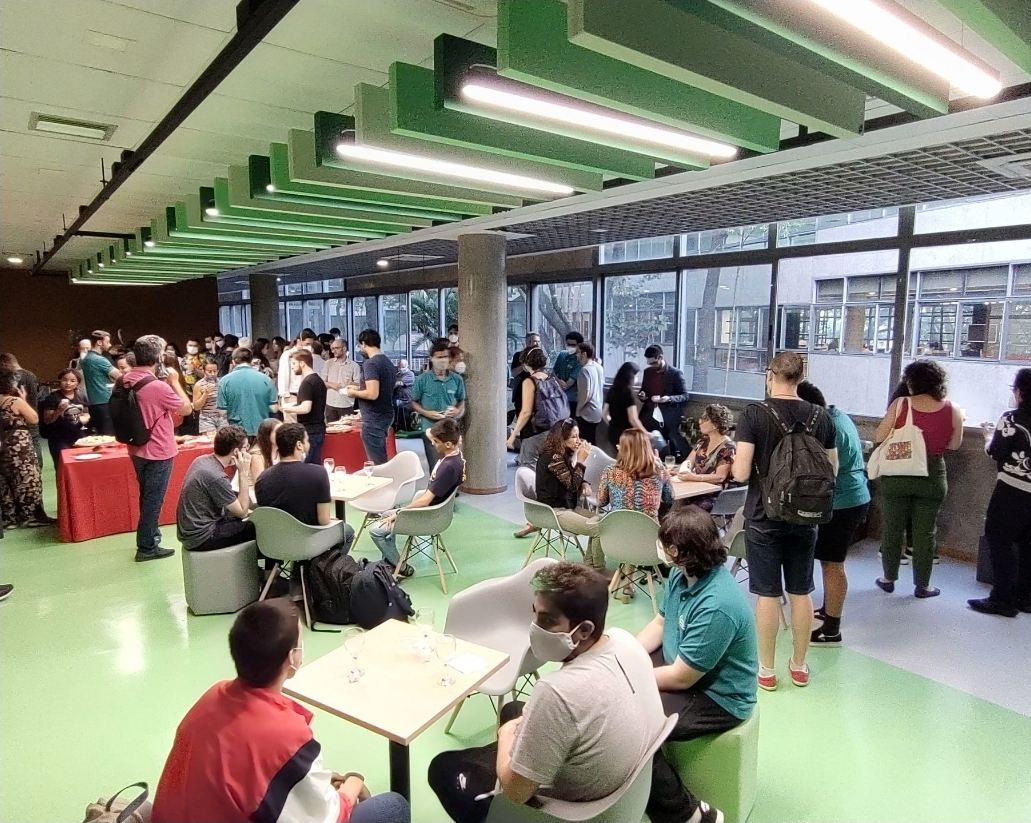
\includegraphics[width=0.6\textwidth]{figuras/cap.1/Screenshot_20260430_160250_Chrome.jpg}
\caption[Café após a Tech Hour do C4AI realizada em 23 de março de 2022, no InovaUSP, primeiro ano do trabalho de campo desta pesquisa.]{Café após a \textit{Tech Hour} do C4AI realizada em 23 de março de 2022, no InovaUSP, primeiro ano do trabalho de campo desta pesquisa. Eu apareço em primeiro plano, de costas, com jaqueta vermelha, em conversa com outros dois pesquisadores de graduação do Centro. A imagem registra um dos primeiros encontros presenciais do C4AI após a pandemia. Foi extraída do site do C4AI, disponível em: \protect\url{https://c4ai.inova.usp.br/about.html\#difusao}. Acesso em: 30 abr. 2026. No intervalo de café após a \textit{Tech Hour} (como são chamadas as apresentações de pesquisa presenciais no C4AI, também transmitidas no YouTube), comecei a conhecer alguns dos pesquisadores do Centro. Lembro-me do contexto em que a foto foi tirada e, por isso, consegui buscar no meu caderno de campo a data exata e uma observação importante que registrei sobre a conversa com eles. Perguntaram-me o que eu fazia no C4AI, presumindo que eu fosse da ciência da computação ou de áreas afins, e expliquei que estava ali para estudar o que eles faziam em um centro de inteligência artificial. Com um tom de descoberta, um deles me disse que \protect\enquote{eles} seriam, então, o meu objeto de pesquisa. Concordei. Para eles, era assim que se fazia ciência. Fiquei alguns dias pensando sobre essa conversa, dúvida que o capítulo~\ref{capitulo1} retoma ao tratar dos modos pelos quais os cientistas da computação reconhecem, ou não, as ciências sociais como interlocutoras legítimas. Essa fotografia foi registrada pelo próprio Centro e, ao consultar o site do C4AI tempos depois, descobri que apareço nela, provavelmente fotografada um pouco depois de essa conversa ter acontecido. Uma outra feliz coincidência.}
\label{fig:tech-hour-c4ai}
\end{figure}

